\documentclass[tikz,border=3pt]{standalone}
\usepackage[T1]{fontenc}
\usepackage{mathptmx}
\usetikzlibrary{arrows.meta,calc,backgrounds}
\begin{document}
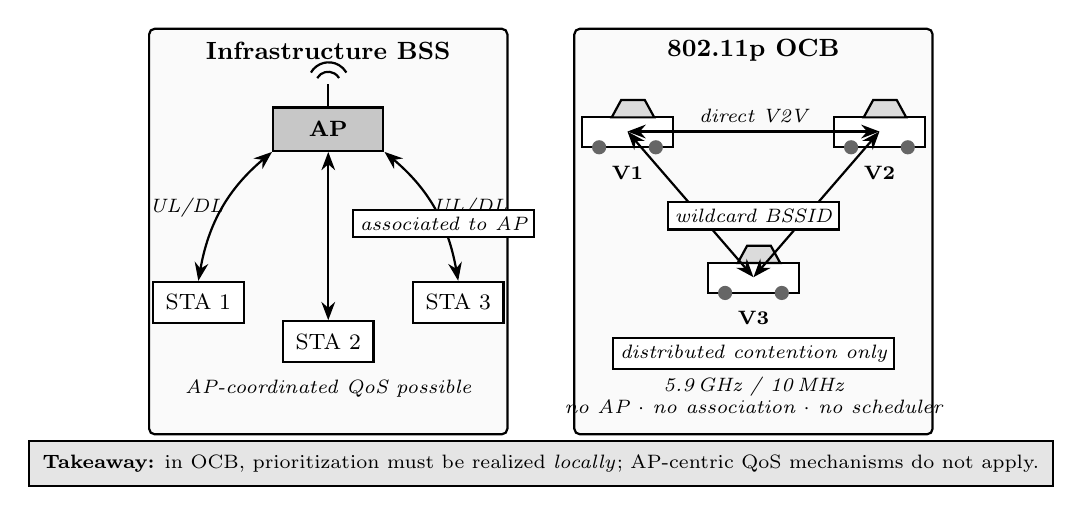
\begin{tikzpicture}[
  font=\footnotesize,
  >=Stealth,
  thick,
  title/.style={font=\small\bfseries},
  lbl/.style={font=\scriptsize\itshape, align=center},
  tag/.style={draw, thick, fill=white, inner sep=2.5pt, font=\scriptsize\itshape, align=center},
  biarr/.style={<->, thick},
  sta/.style={draw, thick, fill=white, minimum width=1.15cm, minimum height=0.52cm, align=center},
]
  % ===================== LEFT: BSS =====================
  \begin{scope}[on background layer]
    \node[draw, thick, rounded corners=2pt, fill=black!2,
          minimum width=4.55cm, minimum height=5.15cm] (pBSS) at (2.15,2.25) {};
  \end{scope}
  \node[title] at (2.15,4.55) {Infrastructure BSS};

  \node[draw, thick, fill=black!22, minimum width=1.40cm, minimum height=0.55cm, align=center]
    (ap) at (2.15,3.55) {\textbf{AP}};
  \draw[thick] (ap.north) -- ++(0,0.28) coordinate (ant);
  \draw[thick] (ant) ++(-0.22,0.15) arc[start angle=150, end angle=30, radius=0.26cm];
  \draw[thick] (ant) ++(-0.14,0.08) arc[start angle=150, end angle=30, radius=0.16cm];

  \node[sta] (s1) at (0.50,1.35) {STA 1};
  \node[sta] (s2) at (2.15,0.85) {STA 2};
  \node[sta] (s3) at (3.80,1.35) {STA 3};

  \draw[biarr] (s1.north) to[out=80, in=220] (ap.south west);
  \draw[biarr] (s2.north) -- (ap.south);
  \draw[biarr] (s3.north) to[out=100, in=-40] (ap.south east);

  \node[lbl] at (0.35,2.55) {UL/DL};
  \node[lbl] at (3.95,2.55) {UL/DL};

  % Tag clear of the centre link
  \node[tag, anchor=west] at (2.45,2.35) {associated to AP};
  \node[lbl] at (2.15,0.25) {AP-coordinated QoS possible};

  % ===================== RIGHT: OCB =====================
  \begin{scope}[shift={(5.40,0)}]
    \begin{scope}[on background layer]
      \node[draw, thick, rounded corners=2pt, fill=black!2,
            minimum width=4.55cm, minimum height=5.15cm] at (2.15,2.25) {};
    \end{scope}
    \node[title] at (2.15,4.55) {802.11p OCB};

    \newcommand{\car}[3]{%
      \begin{scope}[shift={(#2,#3)}]
        \draw[thick, fill=white] (-0.58,-0.08) rectangle (0.58,0.30);
        \draw[thick, fill=black!14]
          (-0.20,0.30) -- (-0.08,0.52) -- (0.22,0.52) -- (0.34,0.30) -- cycle;
        \fill[black!60] (-0.36,-0.08) circle (0.09);
        \fill[black!60] ( 0.36,-0.08) circle (0.09);
        \node[font=\scriptsize\bfseries] at (0,-0.40) {#1};
      \end{scope}
      \coordinate (#1c) at (#2, {#3+0.12});
    }
    \car{V1}{0.55}{3.40}
    \car{V2}{3.75}{3.40}
    \car{V3}{2.15}{1.55}

    \draw[biarr] (V1c) -- (V2c);
    \draw[biarr] (V1c) -- (V3c);
    \draw[biarr] (V2c) -- (V3c);
    \node[lbl] at (2.15,3.72) {direct V2V};

    % Tags as annotations (not hubs)
    \node[tag] at (2.15,2.45) {wildcard BSSID};
    \node[tag] at (2.15,0.70) {distributed contention only};
    \node[lbl] at (2.15,0.28) {5.9\,GHz / 10\,MHz};
    \node[lbl] at (2.15,0.02) {no AP $\cdot$ no association $\cdot$ no scheduler};
  \end{scope}

  \node[draw, thick, fill=black!10, inner sep=5pt, align=center, font=\scriptsize]
    at (4.85,-0.70)
    {\textbf{Takeaway:} in OCB, prioritization must be realized \emph{locally};
     AP-centric QoS mechanisms do not apply.};
\end{tikzpicture}
\end{document}
